\documentclass{article}
\usepackage{graphicx} % Required for inserting images
\usepackage{graphicx} % Required for inserting images
\usepackage[ngerman]{babel}
\usepackage{enumitem}
\usepackage{float}
\usepackage{chngcntr}
\usepackage{glossaries}
\usepackage{tabularx}
\usepackage{hyperref}
\usepackage{titletoc}
\counterwithin{figure}{section}
\counterwithin{table}{section}
\setlength\parindent{0pt}

\makeglossaries

\newglossaryentry{Attributsableitung}
{
    name=Attributsableitung,
    description={Besteht aus einem Namen und einer Ableitung aus existierenden Spalten der Tabelle oder anderen Attributsableitungen.}
}

\newglossaryentry{Alternative}
{
    name=Alternative,
    description={Ein alternatives Verkehrsmittel im Modell. Besteht aus einem Namen und einer Nutzenfunktion, die i.Allg. Referenzen auf Attribute oder Attributsableitungen besitzt.}
}

\newglossaryentry{Projektdatei}
{
    name=Projektdatei,
    description={Enthält potentiell eine CSV-Datei, sowie eventuell Attributsableitungen, Alternativen und vorherige Ergebnisse.}
}

\newglossaryentry{Valide Attributsableitung}
{
    name=Valide Attributsableitung,
    description={Eine Attributsableitung, dessen Name eindeutig ist, die syntaktisch korrekt ist und dessen Referenzen auf Attribute alle existieren.}
}

\newglossaryentry{Invalide Attributsableitung}
{
    name=Valide Attributsableitung,
    description={Eine Attributsableitung, dessen Name bereits vorkommt, die syntaktisch inkorrekt ist oder die eine Referenz auf ein nicht-existierendes Attribut hat.}
}

\newglossaryentry{Valide Alternative}
{
    name=Valide Alternative,
    description={Eine Alternative, dessen Name eindeutig ist, dessen Nutzenfunktion syntaktisch korrekt ist und dessen Referenzen auf Attribute alle existieren.}
}

\newglossaryentry{Invalide Alternative}
{
    name=Invalide Alternative,
    description={Eine Alternative, dessen Name bereits vorkommt, dessen Nutzenfunktion syntaktisch inkorrekt ist oder die eine Referenz auf ein nicht-existierendes Attribut hat.}
}

\newacronym{Ableitung}{Ableitung}{Attributsableitung}

\newacronym{WK}{WK}{Wunschkriterium}

\newacronym{CSV}{CSV}{Comma-separated values}

\newacronym{JSON}{JSON}{JavaScript Object Notation}


\title{Entwurf \\ \large Discrete Choice Model Builder}
\author{Kevin Boehnke \\ \texttt{uxpkw@student.kit.edu}
\and Floriane Bresser \\ \texttt{uspvq@student.kit.edu}
\and Damian Reich \\ \texttt{uqppn@student.kit.edu}
\and Alissa Saleh \\ \texttt{unmbc@student.kit.edu}
\and Michael Schur \\ \texttt{ufkmz@student.kit.edu}}
\date{23. Juni 2023}

\begin{document}

\maketitle
\newpage
\startcontents[maintableofcontents]
\printcontents[maintableofcontents]{}{1}[2]{\section*{Inhaltsverzeichnis}}
\thispagestyle{empty}
\newpage
\pagenumbering{arabic}

\section{Einleitung}


\section{Paketstruktur}
\begin{figure}[H]%
    \centering
    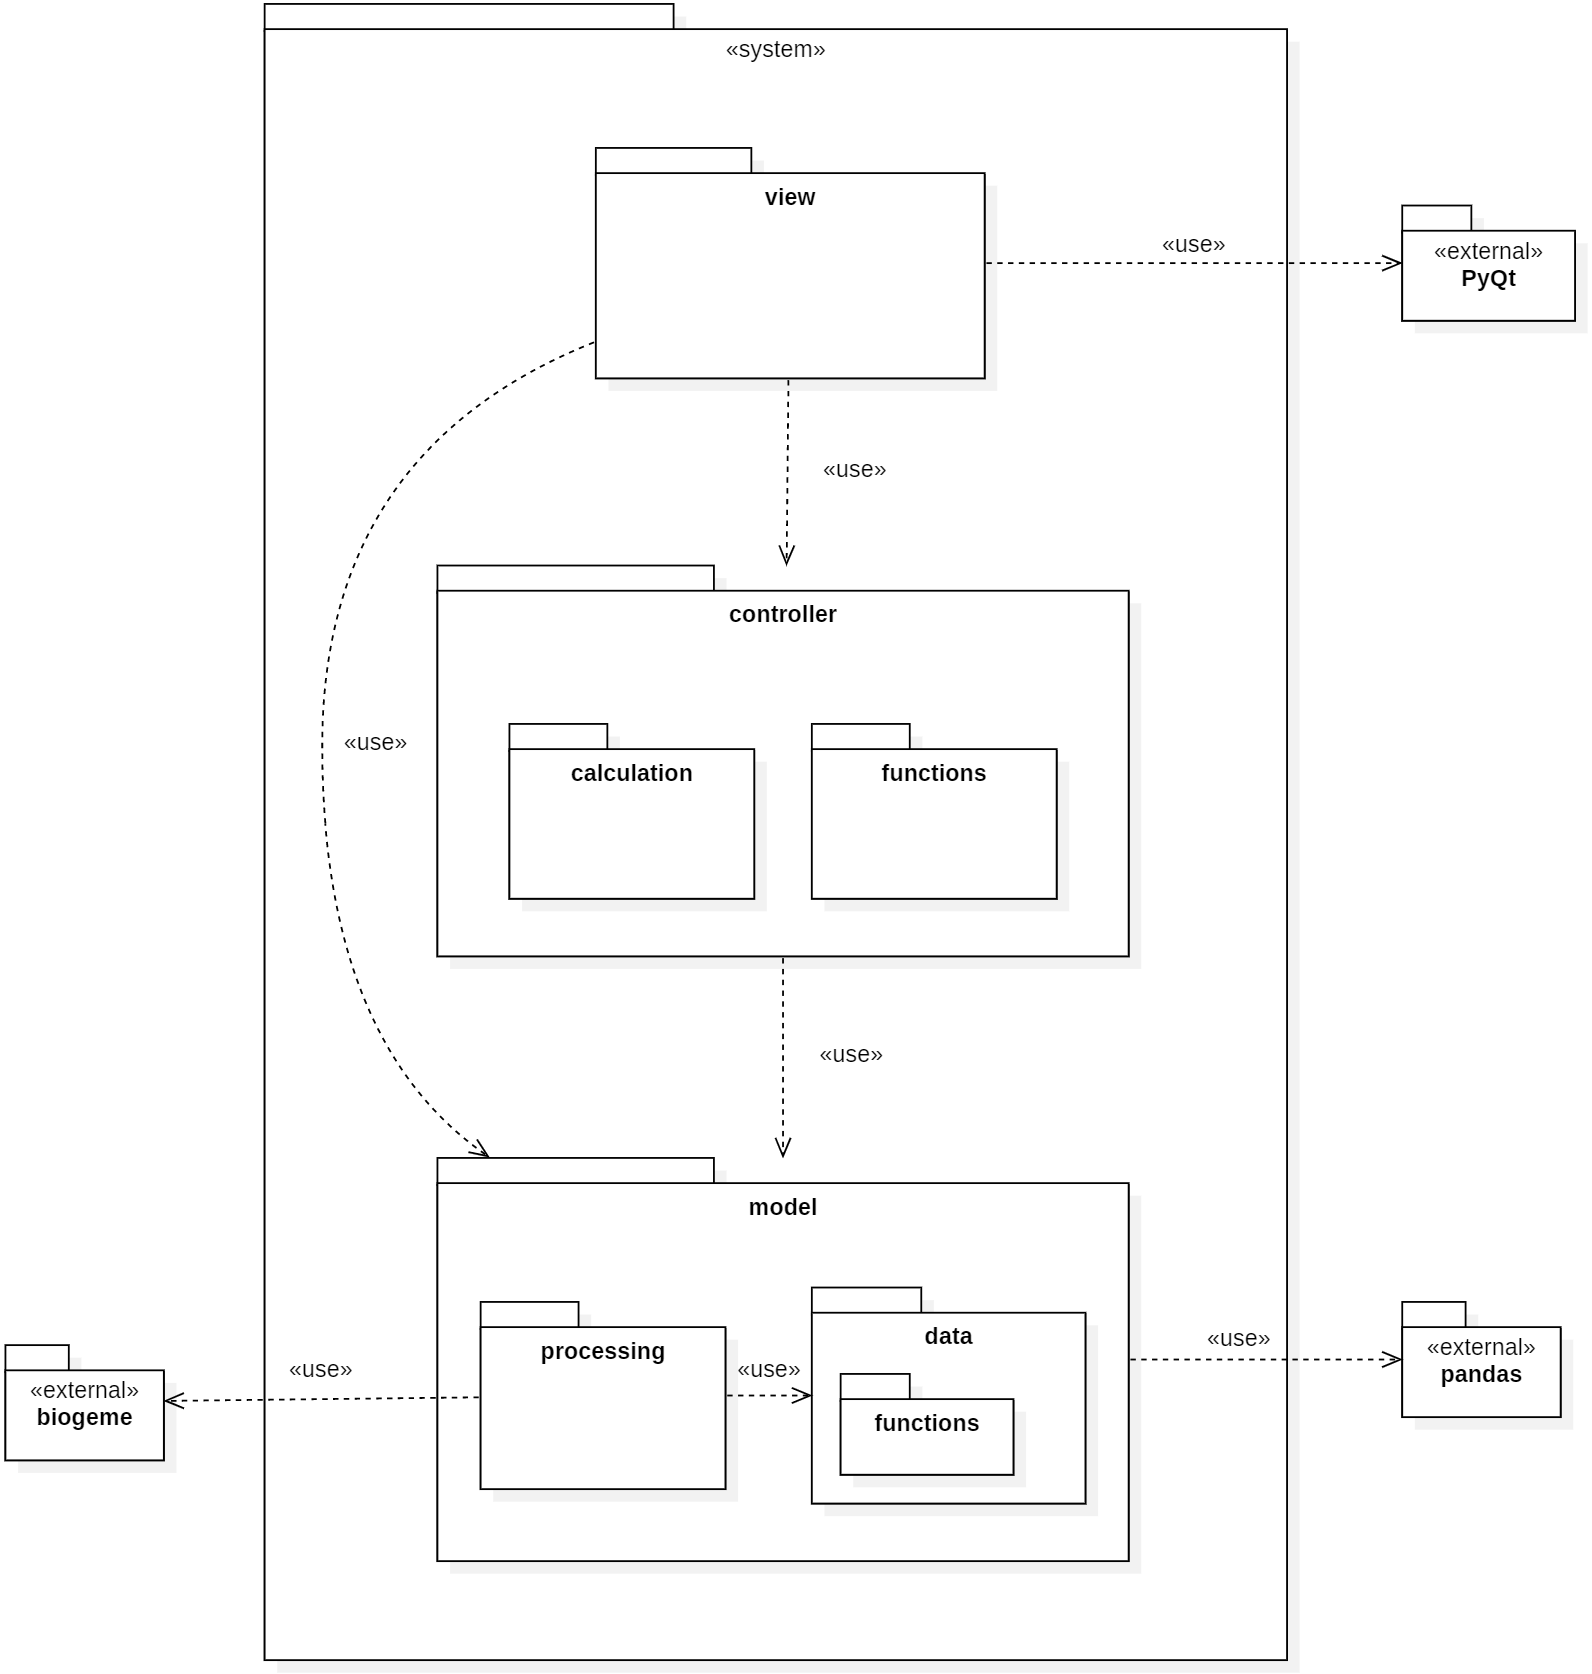
\includegraphics[width=13cm]{img/PackageDiagram.png}
    \caption{Paketdiagramm}
\end{figure}

- Die Software ist eine MVC-Architektur und setzt sich zusammen aus der View, dem Controller und dem Model.
\subsection{View}
- Die View ist verantwortlich für die visuelle Präsentation der im Model vorhandenen Daten. Dafür greift die View auf das externe Paket PyQt zu, welches für die Erstellung graphischer Benutzeroberflächen verwendet wird.
\subsection{Controller}
- Die Controller sind dafür zuständig, die Nutzereingaben aus der View an das Model weiterzuleiten.\\
- Finden Änderungen am Model statt, so senden die betroffenen Klassen der View update-Aufrufe über die Controller aus. Dabei werden die Daten im Model zurückgegeben.\\
- Calculation-Paket: Controller, die für die gesamte Funktionalität der Berechnung aufgerufen werden\\
- Functions-Paket: Controller, die für die Bearbeitung von Alternativen und Attributsableitungen aufgerufen werden
\subsection{Model}
- Das Model umfasst die Datenhaltung bei einem geöffneten Projekt. \\
- Bei Änderungen ist das Model zudem verantwortlich vergangene Eingaben zu speichern. Diese sollen anhand einer undo-/redo-Funktion wieder aufrufbar sein.\\
- Processing-Paket: Umschließt die Funktionalität, welche mit der Konfiguration der Berechnung oder dem Ergebnis zu tun hat. Hier existiert eine Schnittstelle, über welche die tatsächliche Berechnung stattfinden kann. Hier wird standardmäßig das Python Paket \textit{biogeme} verwendet. \\
- Data-Paket: Bezieht alle Klassen mit ein, die für die Datenhaltung des Modells zuständig sind. \\
- Das Python Paket \textit{pandas} wird für die Haltung tabellarischer, vom Nutzer nicht veränderbarer Daten verwendet.


\newpage
\section{Klassenstruktur}
\subsection{View}
\begin{figure}[H]%
    \centering
    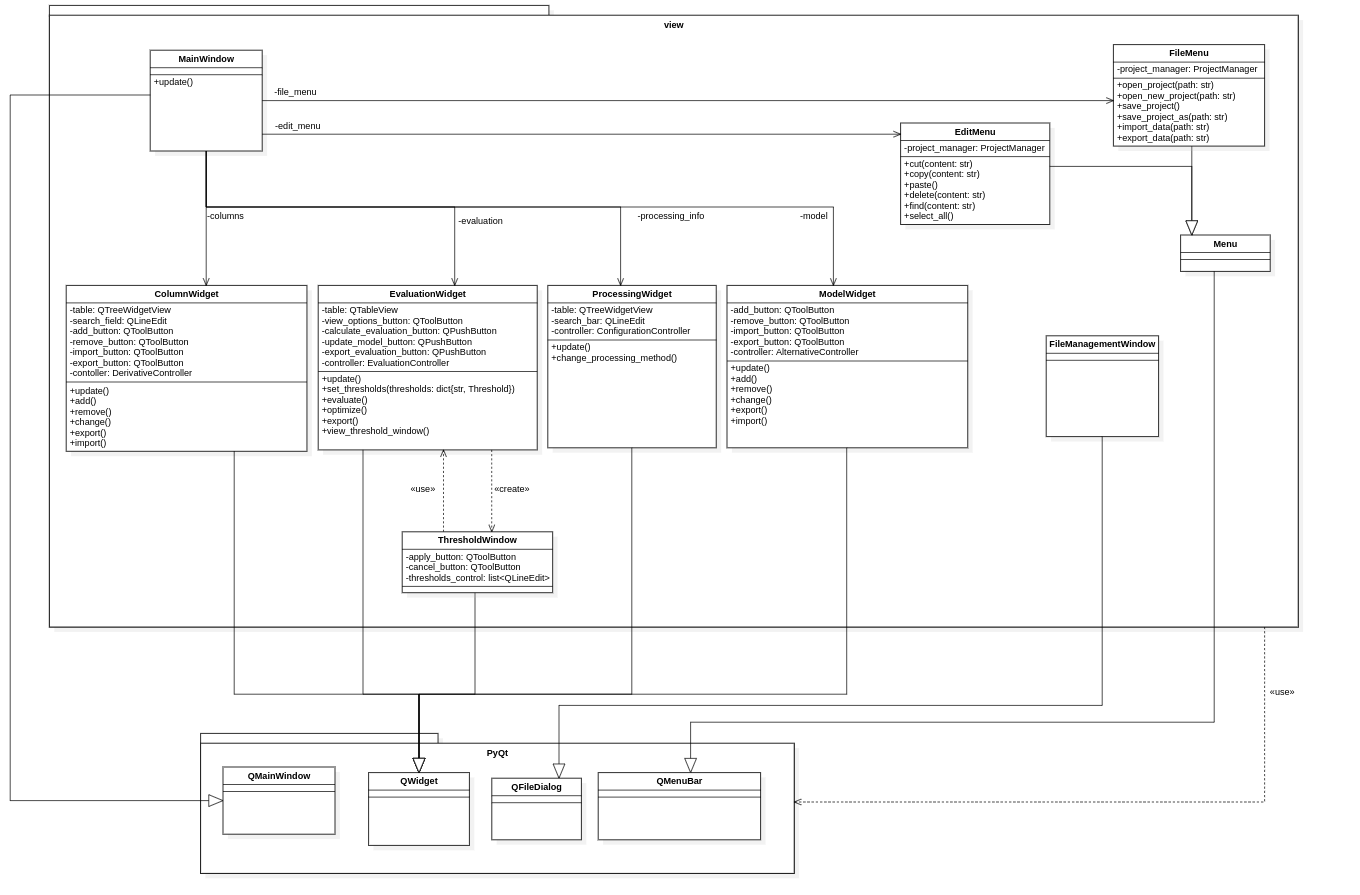
\includegraphics[width=15cm]{entwurf/Entwurf_dokument/img/Alissa/View.png}
    \caption{Das Paket View und seine Klassen mit dem PyQt Paket}
\end{figure}
Im Paket View sind alle Funktionalitäten enthalten, die zur Realisierung der GUI beitragen. Für die graphische Schnittstelle wird PyQt benutzt. Aus diesem Grund erben die Klassen in dem View ihre Funktionalität und Strucktur aus Klassen in PyQt Paket. Im folgenden erfolgt die ausführliche Beschreibung und Erklärung der einzelnen Klassen.

\newpage
\textbf{\large{MainWindow}}\\\\
\begin{figure}[H]%
    \centering
    \begin{minipage}[b]{0.4\textwidth}
        \centering
        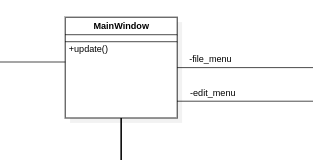
\includegraphics[width=8cm]{entwurf/Entwurf_dokument/img/Alissa/MainWindow.png}
        \caption{Die Klasse MainMenu}
    \end{minipage}
    \hfill
    \begin{minipage}[b]{0.4\textwidth}
        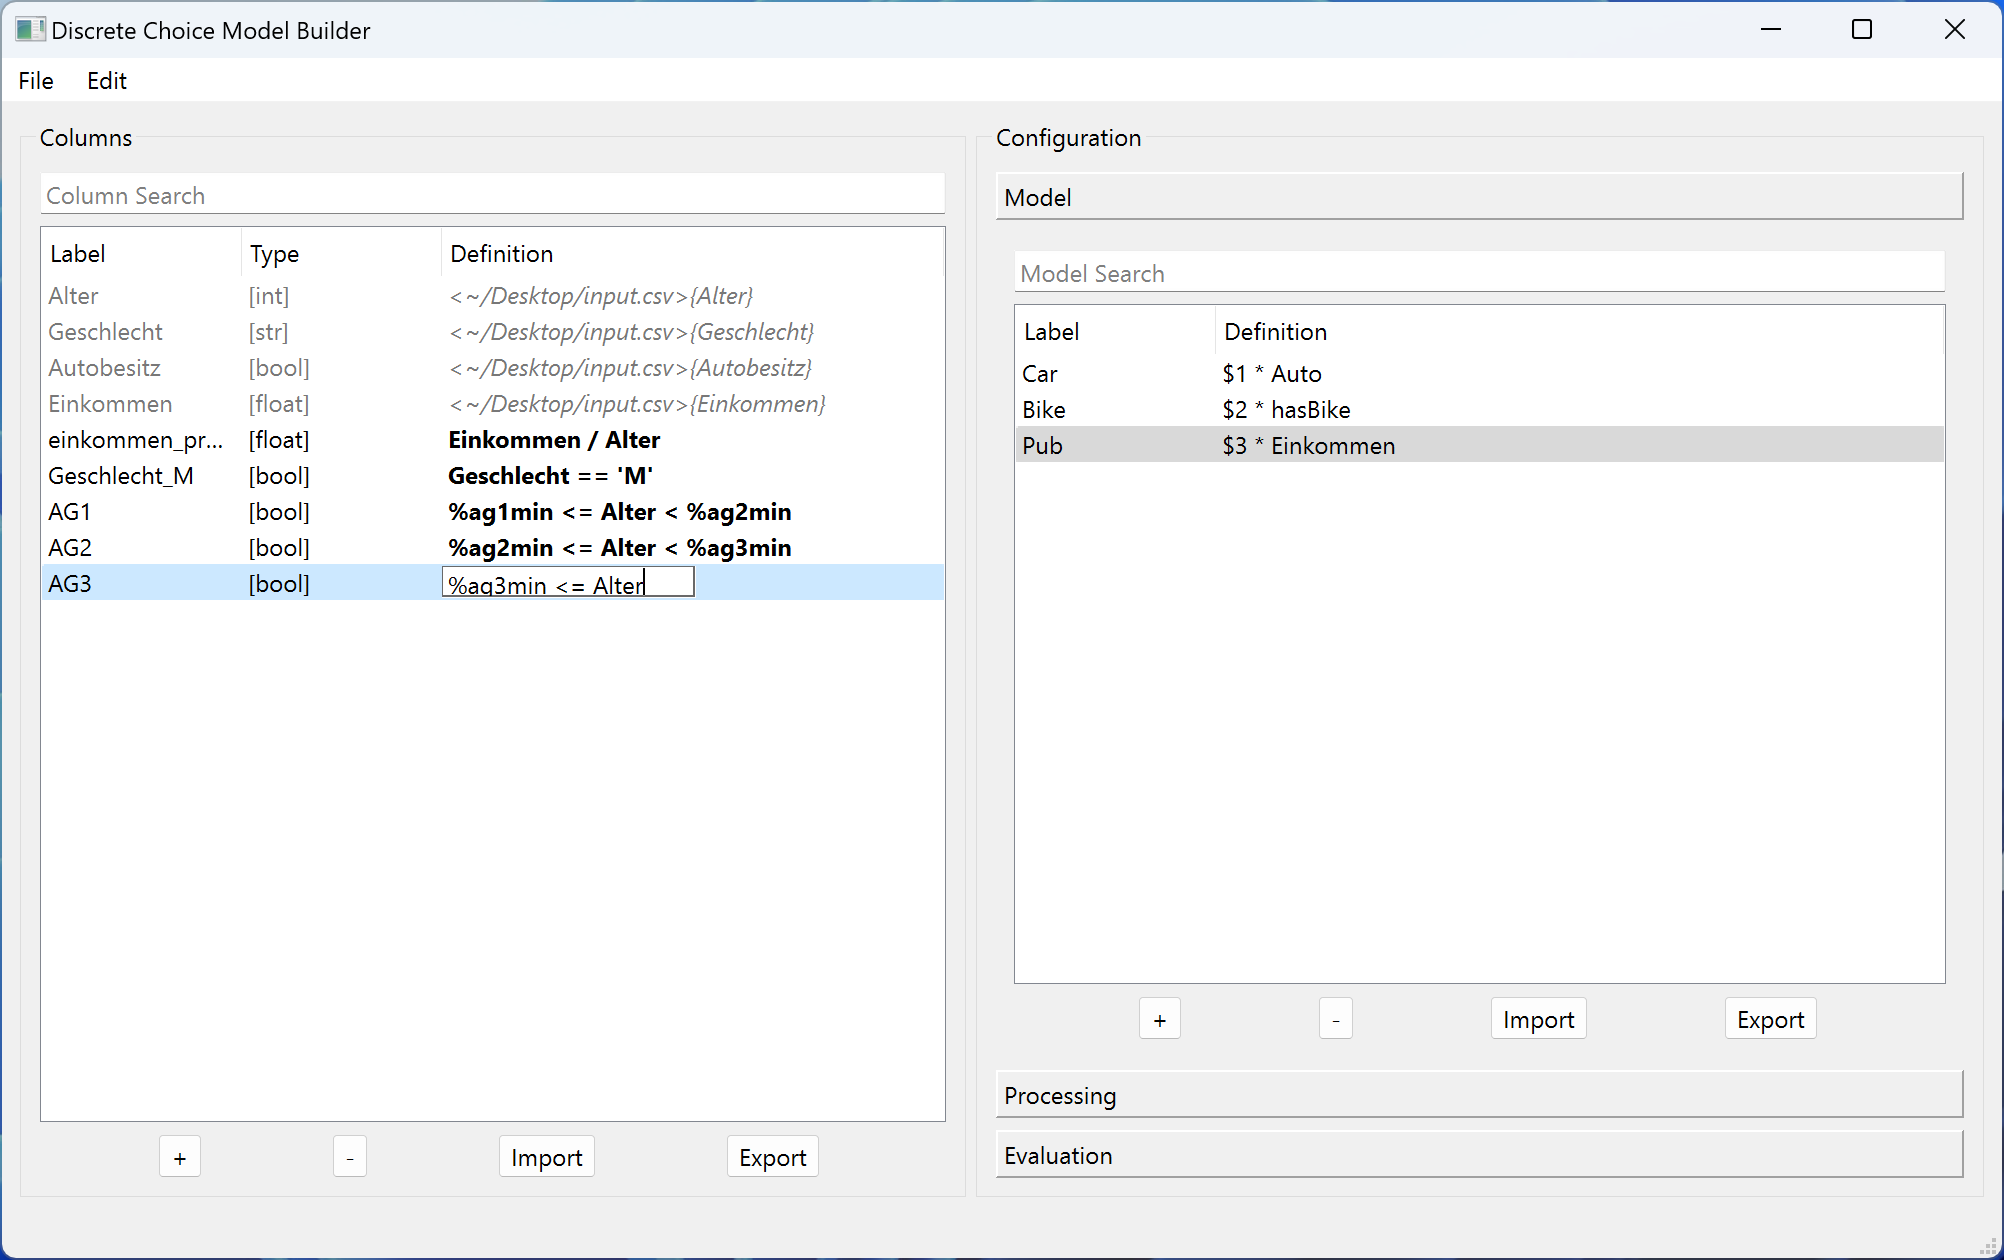
\includegraphics[width=8cm]{specifications/img/gui-screenshots/columns-editing+model.png}
        \caption{Die Klasse MainMenu}
    \end{minipage}
\end{figure}
Dies repräsentiert das Hauptfenster. In dem befinden sich alle graphischen Elemente (Bspw. Tabellen, Menüs, Knöpfe usw.) Die einzelnen Elemente werden je in ihre eigene Klasse spezifiziert, dies erleichtert die Refaktorisierung und das nachträgliche Hinzufügen neuer graphischen Elemente.

Die Klasse erbt von PyQt-QMainWindow. Weitere Informationen finden Sie in der entsprechenden \href[https://doc.qt.io/qt-6/qmainwindow.html]{PyQt-Docs}
\newline \newline

\textbf{{Attribute}}
\begin{itemize}
\item \texttt{file\char`_menu} \newline Repräsentiert das \textit{File Menu} in der GUI
\item \texttt{edit\char`_menu} \newline Repräsentiert das \textit{Edit Menu} in der GUI
\item \texttt{columns} \newline Repräsentiert die Tabelle mit den eigentlichen Daten und Ableitungen. In der GUI befindet sie sich links im Hauptfenster.
\item \texttt{evaluation} \newline Repräsentiert das Teilfenster, wo die Ergebnisse der Berechnungen gezeigt werden.
\item \texttt{processing\char`_info} \newline Repräsentiert 
\item \texttt{model} \newline Beschreibung
\end{itemize}

\textbf{{Methoden}}
\begin{itemize}
\item \texttt{update()} \newline Dient zur Aktualisierung der GUI, wenn ein Befehl aus dem \textit{File Menu} oder \textit{Edit Menu} ausgefüht wird und dies die angezeigten Daten ändert.
\\\\
\underline{{Parameter}}
\begin{tabular}{lll}
 keine \\
\end{tabular}

\underline{{Rückgabewert}}
\begin{tabular}{lll}
 keine \\
\end{tabular}
\end{itemize}

\newpage
\textbf{\large{Menu}}\\\\
\begin{figure}[H]%
    \centering
    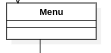
\includegraphics[width=5cm]{entwurf/Entwurf_dokument/img/Alissa/Menu.png}
    \caption{Die Klasse Menu}
\end{figure}
Dies steht für eine Menü in der Menüleiste. Die einzelnen Menüs haben gemeinsame Eigenschaften (gleiche grobe Strucktur), aber jede Menü bietet dem Nutzer unterschiedliche Operationen. Aus diesem Grund wird für jede spezielle Menü eine eigene Klasse erstellt.
Die Klasse \textit{Menu} erbt von PyQt-QMenuBar. Für weitere Informationen sehen Sie \href[https://doc.qt.io/qtforpython-5/PySide2/QtWidgets/QMenuBar.html]{PyQt-Docs}
\newline \newline

\textbf{{Attribute}}
\begin{itemize}
    keine eigene Attribute \newline
\end{itemize}
    
\textbf{{Methoden}}
\begin{itemize}
    keine eigene Methoden
\end{itemize}

\newpage
\textbf{\large{FileMenu}}\\\\
\begin{figure}[H]%
    
    \centering
    \begin{minipage}[b]{0.4\textwidth}
        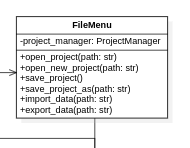
\includegraphics[width=8cm]{entwurf/Entwurf_dokument/img/Alissa/FileMenu.png}
        \caption{Die Klasse FileMenu}
    \end{minipage}
    \hfill
    \begin{minipage}[b]{0.4\textwidth}
        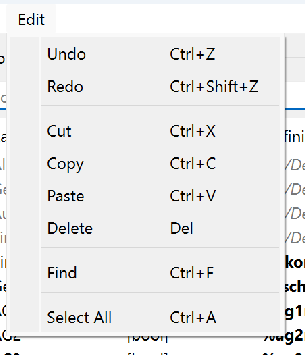
\includegraphics[width=6cm]{entwurf/Entwurf_dokument/img/Alissa/FileMenuGUI.png}
    \caption{Die \textit{File Menu} im GUI. NUR EIN BEISPIEL}
    \end{minipage}
\end{figure}
Die Klasse FileMenu ist die realisierung der \textit{File Menu} aus der graphischen Schnittstelle. Sie erbt ihre grobe Strucktur aus der Klasse \textit{Menu}. Die \textit{File Menu} bietet dem Nutzer die Möglichkeit, das Projekt zu verwalten (importieren, speichern usw.)
\newline \newline

\textbf{{Attribute}}
\begin{itemize}
\item \texttt{project\char`_manager} \newline Das ist der Controller. Mit dem kann die Projekt Verwaltung umgestzt werden.
\end{itemize}

\textbf{{Methoden}}
\begin{itemize}
\item \texttt{open\char`_project} \newline Diese Option ermöglicht dem Nutzer, einen bereitsexistierenden Projekt zu öffnen.
\\\\
\underline{{Parameter}}
\begin{tabular}{lll}
 & \texttt{path} & Der Dateipfad(String), wo das Projekt gespeichert ist. \\
\end{tabular}

\underline{{Rückgabewert}}
\begin{tabular}{lll}
 keine \\
\end{tabular}

\item \texttt{open\char`_new\char`_project} \newline ermöglicht dem Nutzer, eine neues Projekt zu öffnen
\\\\
\underline{{Parameter}}
\begin{tabular}{lll}
 & \texttt{path} & Der Dateipfad(String), wo das Projekt geöffnet und gespeichert werden soll. \\
\end{tabular}

\underline{{Rückgabewert}}
\begin{tabular}{lll}
 keine \\
\end{tabular}

\item \texttt{save\char`_project} \newline ermöglicht dem Nutzer, das geöffnete Projekt zu speichern.
\\\\
\underline{{Parameter}}
\begin{tabular}{lll}
 keine \\
\end{tabular}

\underline{{Rückgabewert}}
\begin{tabular}{lll}
 keine \\
\end{tabular}

\item \texttt{save\char`_project\char`_as} \newline damit kann der Nutzer das geöffnete Projekt, in einem  anderen Dateipfad zu speichern.
\\\\
\underline{{Parameter}}
\begin{tabular}{lll}
 & \texttt{path} & Der Dateipfad(String), wo das Projekt gespeichert werden soll. \\
\end{tabular}

\underline{{Rückgabewert}}
\begin{tabular}{lll}
 keine \\
\end{tabular}

\item \texttt{import\char`_data} \newline Mit dem wird das Laden einer CSV Datei mit den Erhebungsdaten ermöglicht.
\\\\
\underline{{Parameter}}
\begin{tabular}{lll}
 & \texttt{path} & Der Dateipfad, wo der CSV Datei sich befindet. AUch vom Typ String \\
\end{tabular}

\underline{{Rückgabewert}}
\begin{tabular}{lll}
 keine \\
\end{tabular}

\item \texttt{export\char`_data} \newline Mit dieser Option, kann die Tabelle mit den Erhebungsdaten und Ableitungen als eine  Tabelle exportiert werden (Typ)?
\\\\
\underline{{Parameter}}
\begin{tabular}{lll}
 & \texttt{path} & Der Dateipfad(String), wo die CSV Datei exportiert wird. \\
\end{tabular}

\underline{{Rückgabewert}}
\begin{tabular}{lll}
 keine \\
\end{tabular}
\end{itemize}




\newpage
\subsection{Model}
\subsubsection{Data}
\textbf{\large{Model}}\\\\
Abbildung XY

Beschreibung zu \textit{Model}.
\newline \newline

\textbf{{Attribute}}
\begin{itemize}
\item \texttt{data: Data} \newline Beschreibung
\item \texttt{alternatives: dict[label: str, expr: FunctionalExpression]} \newline Beschreibung
\\\\
\end{itemize}

\textbf{{Methoden}}
\begin{itemize}
\item \texttt{set\char`_alternative(label: str, alternative: FunctionalExpression): Model} \newline Beschreibung
\\\\
\underline{{Parameter}}

\begin{tabular}{lll}
 & \texttt{Eingabe} & Beschreibung \\
\end{tabular}

\underline{{Rückgabewert}}

\begin{tabular}{lll}
 & \texttt{Ausgabe} & Beschreibung \\
\end{tabular}

\item \texttt{set\char`_data(data: Data): Model} \newline Beschreibung
\\\\
\underline{{Parameter}}

\begin{tabular}{lll}
 & \texttt{Eingabe} & Beschreibung \\
\end{tabular}

\underline{{Rückgabewert}}

\begin{tabular}{lll}
 & \texttt{Ausgabe} & Beschreibung \\
\end{tabular}
\end{itemize}

\newpage
\textbf{\large{Data}}\\\\
Abbildung XY

Beschreibung zu \textit{Klassenname}.
\newline \newline

\textbf{{Attribute}}
\begin{itemize}
\item \texttt{raw\char`_data: DataFrame} \newline Beschreibung
\item \texttt{derivatives: dict[label: str, expr: FunctionalExpression]} \newline Beschreibung
\\\\
\end{itemize}

\textbf{{Methoden}}
\begin{itemize}
\item \texttt{get\char`_complete\char`_data(): DataFrame} \newline Beschreibung
\\\\
\underline{{Parameter}}

\begin{tabular}{lll}
 & \texttt{Eingabe} & Beschreibung \\
\end{tabular}

\underline{{Rückgabewert}}

\begin{tabular}{lll}
 & \texttt{Ausgabe} & Beschreibung \\
\end{tabular}

\item \texttt{set\char`_raw\char`_data(raw\char`_data: DataFrame): Data} \newline Beschreibung
\\\\
\underline{{Parameter}}

\begin{tabular}{lll}
 & \texttt{Eingabe} & Beschreibung \\
\end{tabular}

\underline{{Rückgabewert}}

\begin{tabular}{lll}
 & \texttt{Ausgabe} & Beschreibung \\
\end{tabular}

\item \texttt{set\char`_derivative(Label: str, derivative: FunctionalExpression): Data} \newline Beschreibung
\\\\
\underline{{Parameter}}

\begin{tabular}{lll}
 & \texttt{Eingabe} & Beschreibung \\
\end{tabular}

\underline{{Rückgabewert}}

\begin{tabular}{lll}
 & \texttt{Ausgabe} & Beschreibung \\
\end{tabular}
\end{itemize}


\newpage
\textbf{\large{FunctionalExpression}}\\\\
Abbildung XY

Beschreibung zu \textit{Klassenname}.
\newline \newline

\textbf{{Attribute}}
\begin{itemize}
\item \texttt{expression: str} \newline Beschreibung
\\\\
\end{itemize}

\textbf{{Methoden}}
\begin{itemize}
\item \texttt{eval(variables: dict)} \newline Beschreibung
\\\\
\underline{{Parameter}}

\begin{tabular}{lll}
 & \texttt{Eingabe} & Beschreibung \\
\end{tabular}

\underline{{Rückgabewert}}

\begin{tabular}{lll}
 & \texttt{Ausgabe} & Beschreibung \\
\end{tabular}

\item \texttt{is\char`_valid(): bool} \newline Beschreibung
\\\\
\underline{{Parameter}}

\begin{tabular}{lll}
 & \texttt{Eingabe} & Beschreibung \\
\end{tabular}

\underline{{Rückgabewert}}

\begin{tabular}{lll}
 & \texttt{Ausgabe} & Beschreibung \\
\end{tabular}

\item \texttt{variables(): set} \newline Beschreibung
\\\\
\underline{{Parameter}}

\begin{tabular}{lll}
 & \texttt{Eingabe} & Beschreibung \\
\end{tabular}

\underline{{Rückgabewert}}

\begin{tabular}{lll}
 & \texttt{Ausgabe} & Beschreibung \\
\end{tabular}

\item \texttt{get\char`_type(): type} \newline Beschreibung
\\\\
\underline{{Parameter}}

\begin{tabular}{lll}
 & \texttt{Eingabe} & Beschreibung \\
\end{tabular}

\underline{{Rückgabewert}}

\begin{tabular}{lll}
 & \texttt{Ausgabe} & Beschreibung \\
\end{tabular}
\end{itemize}


\newpage
\textbf{\large{Interval}}\\\\
Abbildung XY

Beschreibung zu \textit{Klassenname}.
\newline \newline

\textbf{{Attribute}}
\begin{itemize}
\item \texttt{begin: float} \newline Beschreibung
\item \texttt{end: float} \newline Beschreibung
\item \texttt{include\char`_begin: bool} \newline Beschreibung
\item \texttt{include\char`_end: bool} \newline Beschreibung
\\\\
\end{itemize}

\textbf{{Methoden}}
\begin{itemize}
\item \texttt{\char`_\char`_contains\char`_\char`_(other: float): bool} \newline Beschreibung
\\\\
\underline{{Parameter}}

\begin{tabular}{lll}
 & \texttt{Eingabe} & Beschreibung \\
\end{tabular}

\underline{{Rückgabewert}}

\begin{tabular}{lll}
 & \texttt{Ausgabe} & Beschreibung \\
\end{tabular}
\end{itemize}


\newpage
\textbf{\large{GroupMap}}\\\\
Abbildung XY

Beschreibung zu \textit{Klassenname}.
\newline \newline

\textbf{Attribute}
\begin{itemize}
\item \texttt{groups: list} \newline Beschreibung
\\\\
\end{itemize}

\textbf{Methoden}
\begin{itemize}
\item \texttt{\char`_\char`_call\char`_\char`_(element: T): int} \newline Beschreibung
\\\\
\underline{{Parameter}}

\begin{tabular}{lll}
 & \texttt{Eingabe} & Beschreibung \\
\end{tabular}

\underline{Rückgabewert}

\begin{tabular}{lll}
 & \texttt{Ausgabe} & Beschreibung \\
\end{tabular}
\end{itemize}

\newpage
\subsubsection{Processing}

\subsubsection*{\large{\textbf{ProcessingConfig}\label{cls:ProcessingConfig}}}\\
\textit{\flqq{}abstract\frqq} \textit{\flqq{}immutable\frqq}\normalsize\\\\
\begin{tabular}{lll}
 Superklassen: & --\\
 Subklassen: & \texttt{SimpleProcessingConfig}, \texttt{VariedProcessingConfig}
\end{tabular}\\
\begin{figure}[H]%
    \centering
    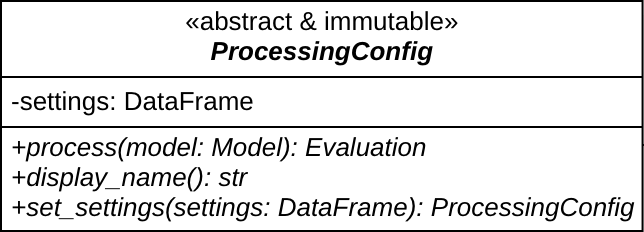
\includegraphics[width=13cm]{entwurf/Entwurf_dokument/img/cls/model/ProcessingConfig.png}
    \caption{Klassendiagramm \texttt{ProcessingConfig}}
\end{figure}

Die Klasse definiert, auf welche Art und Weise eine Datenverarbeitung eines Datenmodells erfolgt.
\\\\

\textbf{Attribute}
\begin{itemize}\setlength\itemsep{3em}
\item \texttt{settings: pandas.DataFrame}\\\\
Datentabelle der Nutzereinstellungen.
\\\\
\end{itemize}

\textbf{Methoden}
\begin{itemize}\setlength\itemsep{3em}
\item \textit{\flqq{}abstract\frqq} \texttt{\textit{process(model: Model): Evaluation}}\\\\
Verarbeitet ein \texttt{model} entsprechend der Konfigurationsklasse und erstellt eine Auswertung vom Typ \texttt{Evaluation}.
\\\\
\underline{Parameter}\\
\begin{tabular}{lll}
 & \texttt{model} & Diskretes Wahlmodell, auf dem eine Verabreitung erfolgen soll.\\
\end{tabular}

\underline{Rückgabewert}\\
\begin{tabular}{lll}
 & Auswertung, wie durch Konfigurationsklasse definiert.\\
\end{tabular}

\underline{Exceptions}\\
\begin{tabular}{lll}
 & \texttt{ValueError} & Modell hat nicht die durch die Konfiguration geforderten Eigenschaften.\\
\end{tabular}

\item \textit{\flqq{}abstract\frqq} \texttt{\textit{display\char`_name(): str}}\\\\
Getter für Anzeigename der Konfigurationsklasse zur Darstellung im Auswahlmenü.
\\\\
\underline{Rückgabewert}\\
\begin{tabular}{lll}
 & Anzeigename als \texttt{str}.\\
\end{tabular}

\item \textit{\flqq{}abstract\frqq} \texttt{\textit{set\char`_settings(settings: pandas.DataFrame): ProcessingConfig}}\\\\
Erstellt eine Kopie des Objekts, in der lediglich das Attribut \texttt{settings} durch das übergebene Attribut überschrieben wird.
\\\\
\underline{Parameter}\\
\begin{tabular}{lll}
 & \texttt{settings} & Neue Datentabelle der Nutzereinstellungen.\\
\end{tabular}

\underline{Rückgabewert}\\
\begin{tabular}{lll}
 & Anzeigename als \texttt{str}.\\
\end{tabular}
\end{itemize}

%----------------------------------
\subsubsection*{\large{\textbf{SimpleProcessingConfig}\label{cls:SimpleProcessingConfig}}}\\
\textit{\flqq{}immutable\frqq}\normalsize\\\\
\begin{tabular}{lll}
 Superklassen: & \texttt{ProcessingConfig}\\
 Subklassen: & --
\end{tabular}\\
\begin{figure}[H]%
    \centering
    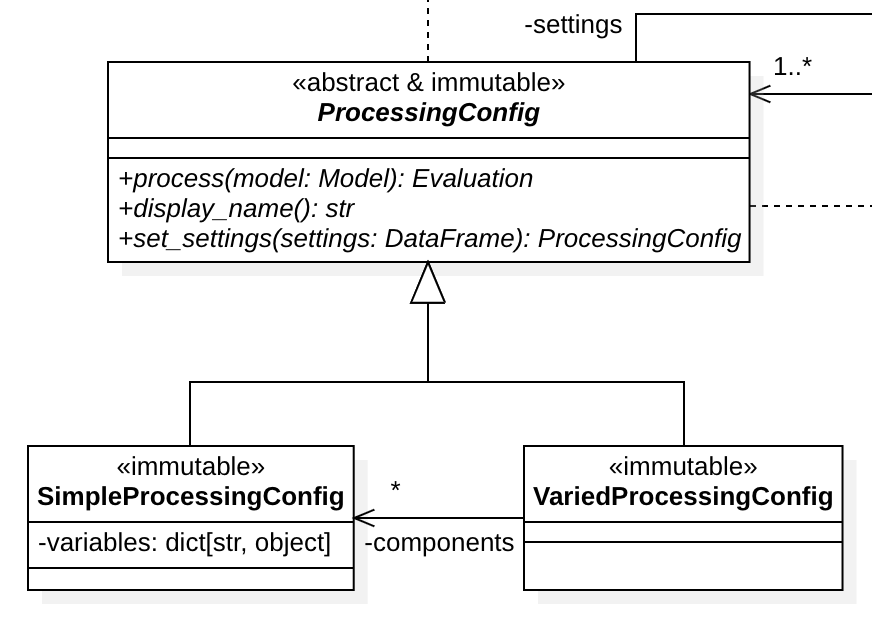
\includegraphics[width=13cm]{entwurf/Entwurf_dokument/img/cls/model/ProcessingConfigs.png}
    \caption{Klassendiagramm aller Subklassen von \texttt{ProcessingConfig}}
\end{figure}

Die Klasse definiert das Verfahren einer einfachen Parameterschätzung eines diskreten Wahlmodells und weist den verbleibenden freie Variablen im Modell einen Wert zu.
\\\\

\textbf{Attribute}
\begin{itemize}\setlength\itemsep{3em}
\item \texttt{variables: dict[str, object]}\\\\
Zuordnung zwischen verbleibenden freien Variablen und einem Wert, der für die Berechnung verwendet werden soll.\\
Der Datentyp der Werte kann nicht weiter eingeschränkt werden, da dieser von der Verwendung der freien Variablen abhängt.
\\\\
\end{itemize}

\textbf{Methoden}
\begin{itemize}\setlength\itemsep{3em}
\item \texttt{process(model: Model): Evaluation}\\\\
Wendet die definierte Parameterschätzung auf \texttt{model} an und erstellt eine Auswertung vom Typ \texttt{Evaluation}.
\\\\
\underline{Parameter}\\
\begin{tabular}{lll}
 & \texttt{model} & Diskretes Wahlmodell, auf dem eine Verabreitung erfolgen soll.\\
\end{tabular}

\underline{Rückgabewert}\\
\begin{tabular}{lll}
 & Auswertung, wie durch Konfigurationsklasse definiert.\\
\end{tabular}

\underline{Exceptions}\\
\begin{tabular}{lll}
 & \texttt{ValueError} & Modell hat nicht die durch die Konfiguration geforderten Eigenschaften.\\
\end{tabular}
\end{itemize}

%----------------------------------
\subsubsection*{\large{\textbf{VariedProcessingConfig}\label{cls:VariedProcessingConfig}}}\\
\textit{\flqq{}immutable\frqq}\normalsize\\\\
\begin{tabular}{lll}
 Superklassen: & \texttt{ProcessingConfig}\\
 Subklassen: & --
\end{tabular}\\
\begin{figure}[H]%
    \centering
    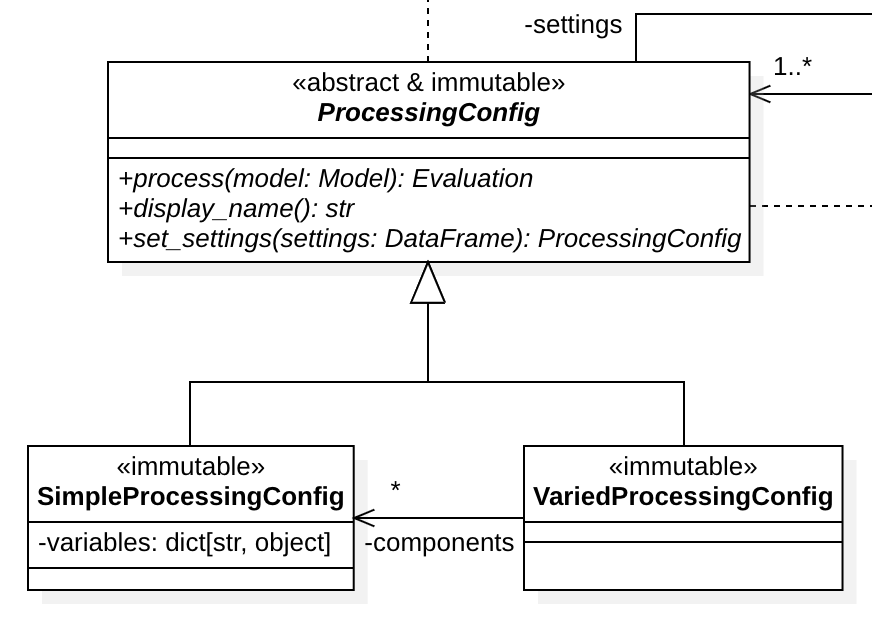
\includegraphics[width=13cm]{entwurf/Entwurf_dokument/img/cls/model/ProcessingConfigs.png}
    \caption{Klassendiagramm aller Subklassen von \texttt{ProcessingConfig}}
\end{figure}

Die Klasse definiert eine mehrfache Anwendung einer Parameterschätzung eines diskreten Wahlmodells und weist dabei den verbleibenden freie Variablen im Modell je unterschiedliche Werte zu. Die Werte können definiert werden und müssen vor dem Aufruf von \texttt{process} vorliegen.
\\\\

\textbf{Attribute}
\begin{itemize}\setlength\itemsep{3em}
\item \texttt{components: list[SimpleProcessingConfig]}\\\\
Liste von Konfigurationen vom Typ \texttt{SimpleProcessingConfig}, die nacheinander ausgeführt werden sollen.
\\\\
\end{itemize}

\textbf{Methoden}
\begin{itemize}\setlength\itemsep{3em}
\item \texttt{process(model: Model): Evaluation}\\\\
Wendet alle hinterlegten einzelnen Parameterschätzungen auf \texttt{model} an und erstellt eine Auswertung vom Typ \texttt{Evaluation}.
\\\\
\underline{Parameter}\\
\begin{tabular}{lll}
 & \texttt{model} & Diskretes Wahlmodell, auf dem eine Verabreitung erfolgen soll.\\
\end{tabular}

\underline{Rückgabewert}\\
\begin{tabular}{lll}
 & Auswertung, wie durch Konfigurationsklasse definiert.\\
\end{tabular}

\underline{Exceptions}\\
\begin{tabular}{lll}
 & \texttt{ValueError} & Modell hat nicht die durch die Konfiguration geforderten Eigenschaften.\\
\end{tabular}
\end{itemize}

%----------------------------------
\subsubsection*{\large{\textbf{Evaluation}\label{cls:Evaluation}}}\\
\textit{\flqq{}immutable\frqq}\normalsize\\\\
\begin{tabular}{lll}
 Superklassen: & --\\
 Subklassen: & --
\end{tabular}\\
\begin{figure}[H]%
    \centering
    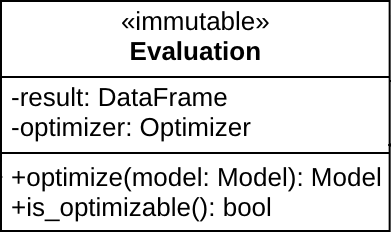
\includegraphics[width=13cm]{entwurf/Entwurf_dokument/img/cls/model/Evaluation.png}
    \caption{Klassendiagramm von \texttt{Evaluation}}
\end{figure}

Die Klasse entspricht der Auswertung einer Parameterschätzung von einem diskreten Wahlmodell.
\\\\

\textbf{Attribute}
\begin{itemize}\setlength\itemsep{3em}
\item \texttt{result: pandas.DataFrame}\\\\
Auswertungstabelle der verwendeten Berechnungsbibliothek oder eine zusammengesetzte Tabelle aus mehreren Auswertungstabellen.
\\\\
\end{itemize}

\textbf{Methoden}
\begin{itemize}\setlength\itemsep{3em}
\item \texttt{optimize(model: Model): Model}\\\\
Falls der Auswertung ein Modelloptimierungsverfahren beiliegt (siehe \texttt{is\char`_optimizable()}), wird das diskrete Wahlmodell dementsprechend verbessert.\\\\
\underline{Parameter}\\
\begin{tabular}{lll}
 & \texttt{model} & Diskretes Wahlmodell, das optimiert werden soll.\\
\end{tabular}

\underline{Rückgabewert}\\
\begin{tabular}{lll}
 & Das optimierte diskrete Wahlmodell.\\
\end{tabular}

\underline{Exceptions}\\
\begin{tabular}{lll}
 & \texttt{ValueError} & Modell hat nicht die durch den Optimierungsalgorithmus geforderten Eigenschaften.\\
\end{tabular}

\item \texttt{is\char`_optimizable(): bool}\\\\
Prüft, ob eine Optimierung auf Grundlage dieser Auswertung prinzipiell möglich ist.\\\\
\underline{Parameter}\\
\begin{tabular}{lll}
 & \texttt{model} & Diskretes Wahlmodell, auf dem eine Optimierung erfolgen soll.\\
\end{tabular}

\underline{Rückgabewert}\\
\begin{tabular}{lll}
 & Wahrheitswert, ob Optimierung auf Grundlage dieser Auswertung prinzipiell möglich ist.\\
\end{tabular}
\end{itemize}

%----------------------------------
\subsubsection*{\large{\textbf{Optimizer}\label{cls:Optimizer}}}\\
\textit{\flqq{}interface\frqq}\normalsize\\\\
\begin{tabular}{lll}
 Superklassen: & --\\
 Subklassen: & --
\end{tabular}\\
\begin{figure}[H]%
    \centering
    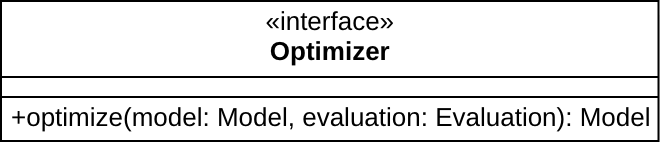
\includegraphics[width=13cm]{entwurf/Entwurf_dokument/img/cls/model/Optimizer.png}
    \caption{Klassendiagramm von \texttt{Optimizer}}
\end{figure}

Das Interface bietet eine Schnittstelle zur Implementierung eines Optimierungsalgorithmus.
\\\\

\textbf{Methoden}
\begin{itemize}\setlength\itemsep{3em}
\item \textit{\flqq{}abstract\frqq} \texttt{\textit{optimize(model: Model, evaluation: Evaluation): Model}}\\\\
Falls der Auswertung ein Modelloptimierungsverfahren beiliegt (siehe \texttt{is\char`_optimizable()}), wird das diskrete Wahlmodell dementsprechend verbessert.\\\\
\underline{Parameter}\\
\begin{tabular}{lll}
 & \texttt{model} & Diskretes Wahlmodell, das optimiert werden soll.\\
 & \texttt{evaluation} & Auswertung, auf deren Grundlage eine Optimierung vorgenommen werden soll.
\end{tabular}

\underline{Rückgabewert}\\
\begin{tabular}{lll}
 & Das optimierte diskrete Wahlmodell.\\
\end{tabular}

\underline{Exceptions}\\
\begin{tabular}{lll}
 & \texttt{ValueError} & Ein Parameter hat nicht die durch den Optimierungsalgorithmus geforderten Eigenschaften.\\
\end{tabular}
\end{itemize}

%----------------------------------
\subsubsection*{\large{\textbf{Project}\label{cls:Project}}}\\
\textit{\flqq{}interface\frqq}\normalsize\\\\
\begin{tabular}{lll}
 Superklassen: & \texttt{ProcessingConfig}\\
 Subklassen: & --
\end{tabular}\\
\begin{figure}[H]%
    \centering
    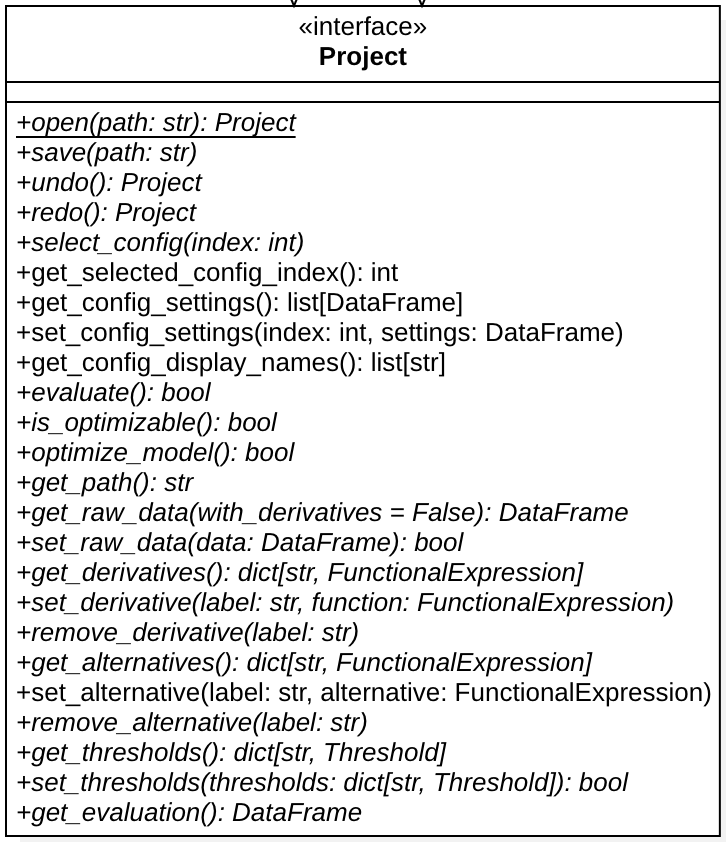
\includegraphics[width=13cm]{entwurf/Entwurf_dokument/img/cls/model/Project.png}
    \caption{Klassendiagramm von \texttt{Project}}
\end{figure}

Das Interface stellt die Schnittstelle zwischen Datenmodell (\emph{Model}) und Benutzeroberfläche (\emph{View} und \emph{Controller}) dar. Es beinhaltet alle benötigten Methoden zur vollständigen Verwaltung eines Projekts.
\\\\

\textbf{Methoden}
\begin{itemize}\setlength\itemsep{3em}
\item \textit{\flqq{}static\frqq} \texttt{\underline{open(path: str): Project}}\\\\
Lädt ein unter \texttt{path} gespeichertes Projekt.
\\\\
\underline{Parameter}\\
\begin{tabular}{lll}
 & \texttt{path} & Dateipfad des Projekts.\\
\end{tabular}

\underline{Rückgabewert}\\
\begin{tabular}{lll}
 & Interface des Projekts.\\
\end{tabular}

\underline{Exceptions}\\
\begin{tabular}{lll}
 & \texttt{ValueError} & Dateipfad ist ungültig.\\
 & \texttt{IOError} & Fehler bei I/O-Operation.\\
\end{tabular}

\item \textit{\flqq{}static\frqq} \texttt{\underline{open(path: str): Project}}\\\\
Lädt ein unter \texttt{path} gespeichertes Projekt.
\\\\
\underline{Parameter}\\
\begin{tabular}{lll}
 & \texttt{path} & Dateipfad des Projekts.\\
\end{tabular}

\underline{Rückgabewert}\\
\begin{tabular}{lll}
 & Interface des Projekts.\\
\end{tabular}

\underline{Exceptions}\\
\begin{tabular}{lll}
 & \texttt{ValueError} & Dateipfad ist ungültig.\\
 & \texttt{IOError} & Fehler bei I/O-Operation.\\
\end{tabular}

\item \texttt{process(model: Model): Evaluation}\\\\
Wendet die definierte Parameterschätzung auf \texttt{model} an und erstellt eine Auswertung vom Typ \texttt{Evaluation}.
\\\\
\underline{Parameter}\\
\begin{tabular}{lll}
 & \texttt{model} & Beschreibung.\\
\end{tabular}

\underline{Rückgabewert}\\
\begin{tabular}{lll}
 & Beschreibung.\\
\end{tabular}

\underline{Exceptions}\\
\begin{tabular}{lll}
 & \texttt{ValueError} & Ein Parameter hat nicht die geforderten Eigenschaften.\\
\end{tabular}
\end{itemize}

%----------------------------------
\subsubsection*{\large{\textbf{ProjectSnapshot}\label{cls:ProjectSnapshot}}}\\
\textit{\flqq{}immutable\frqq}\normalsize\\\\
\begin{tabular}{lll}
 Superklassen: & \texttt{ProcessingConfig}\\
 Subklassen: & --
\end{tabular}\\
\begin{figure}[H]%
    \centering
    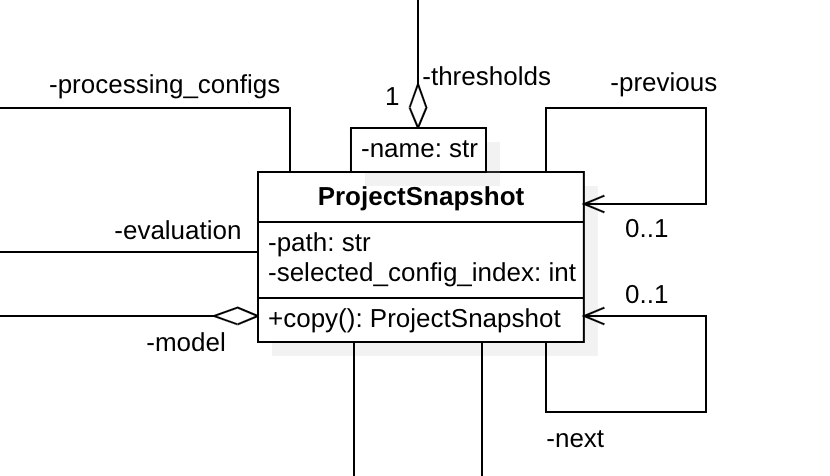
\includegraphics[width=13cm]{entwurf/Entwurf_dokument/img/cls/model/ProjectSnapshot.png}
    \caption{Klassendiagramm aller Subklassen von \texttt{ProcessingConfig}}
\end{figure}

Die Klasse definiert das Verfahren einer einfachen Parameterschätzung eines diskreten Wahlmodells und weist den verbleibenden freie Variablen im Modell einen Wert zu.
\\\\

\textbf{Attribute}
\begin{itemize}\setlength\itemsep{3em}
\item \texttt{variables: dict[str, object]}\\\\
Zuordnung zwischen verbleibenden freien Variablen und einem Wert, der für die Berechnung verwendet werden soll.\\
Der Datentyp der Werte kann nicht weiter eingeschränkt werden, da dieser von der Verwendung der freien Variablen abhängt.
\\\\
\end{itemize}

\textbf{Methoden}
\begin{itemize}\setlength\itemsep{3em}
\item \texttt{process(model: Model): Evaluation}\\\\
Wendet die definierte Parameterschätzung auf \texttt{model} an und erstellt eine Auswertung vom Typ \texttt{Evaluation}.
\\\\
\underline{Parameter}\\
\begin{tabular}{lll}
 & \texttt{model} & Diskretes Wahlmodell, auf dem eine Verabreitung erfolgen soll.\\
\end{tabular}

\underline{Rückgabewert}\\
\begin{tabular}{lll}
 & Auswertung, wie durch Konfigurationsklasse definiert.\\
\end{tabular}

\underline{Exceptions}\\
\begin{tabular}{lll}
 & \texttt{ValueError} & Modell hat nicht die durch die Konfiguration geforderten Eigenschaften.\\
\end{tabular}
\end{itemize}

\newpage
\subsection{Controller}

Im folgenden Abschnitt werden die Klassen des Paketes \emph{Controller}, so wie sie in Abb.~3.1 dargestellt sind, dokumentiert.

\begin{figure}[H]%
    \centering
    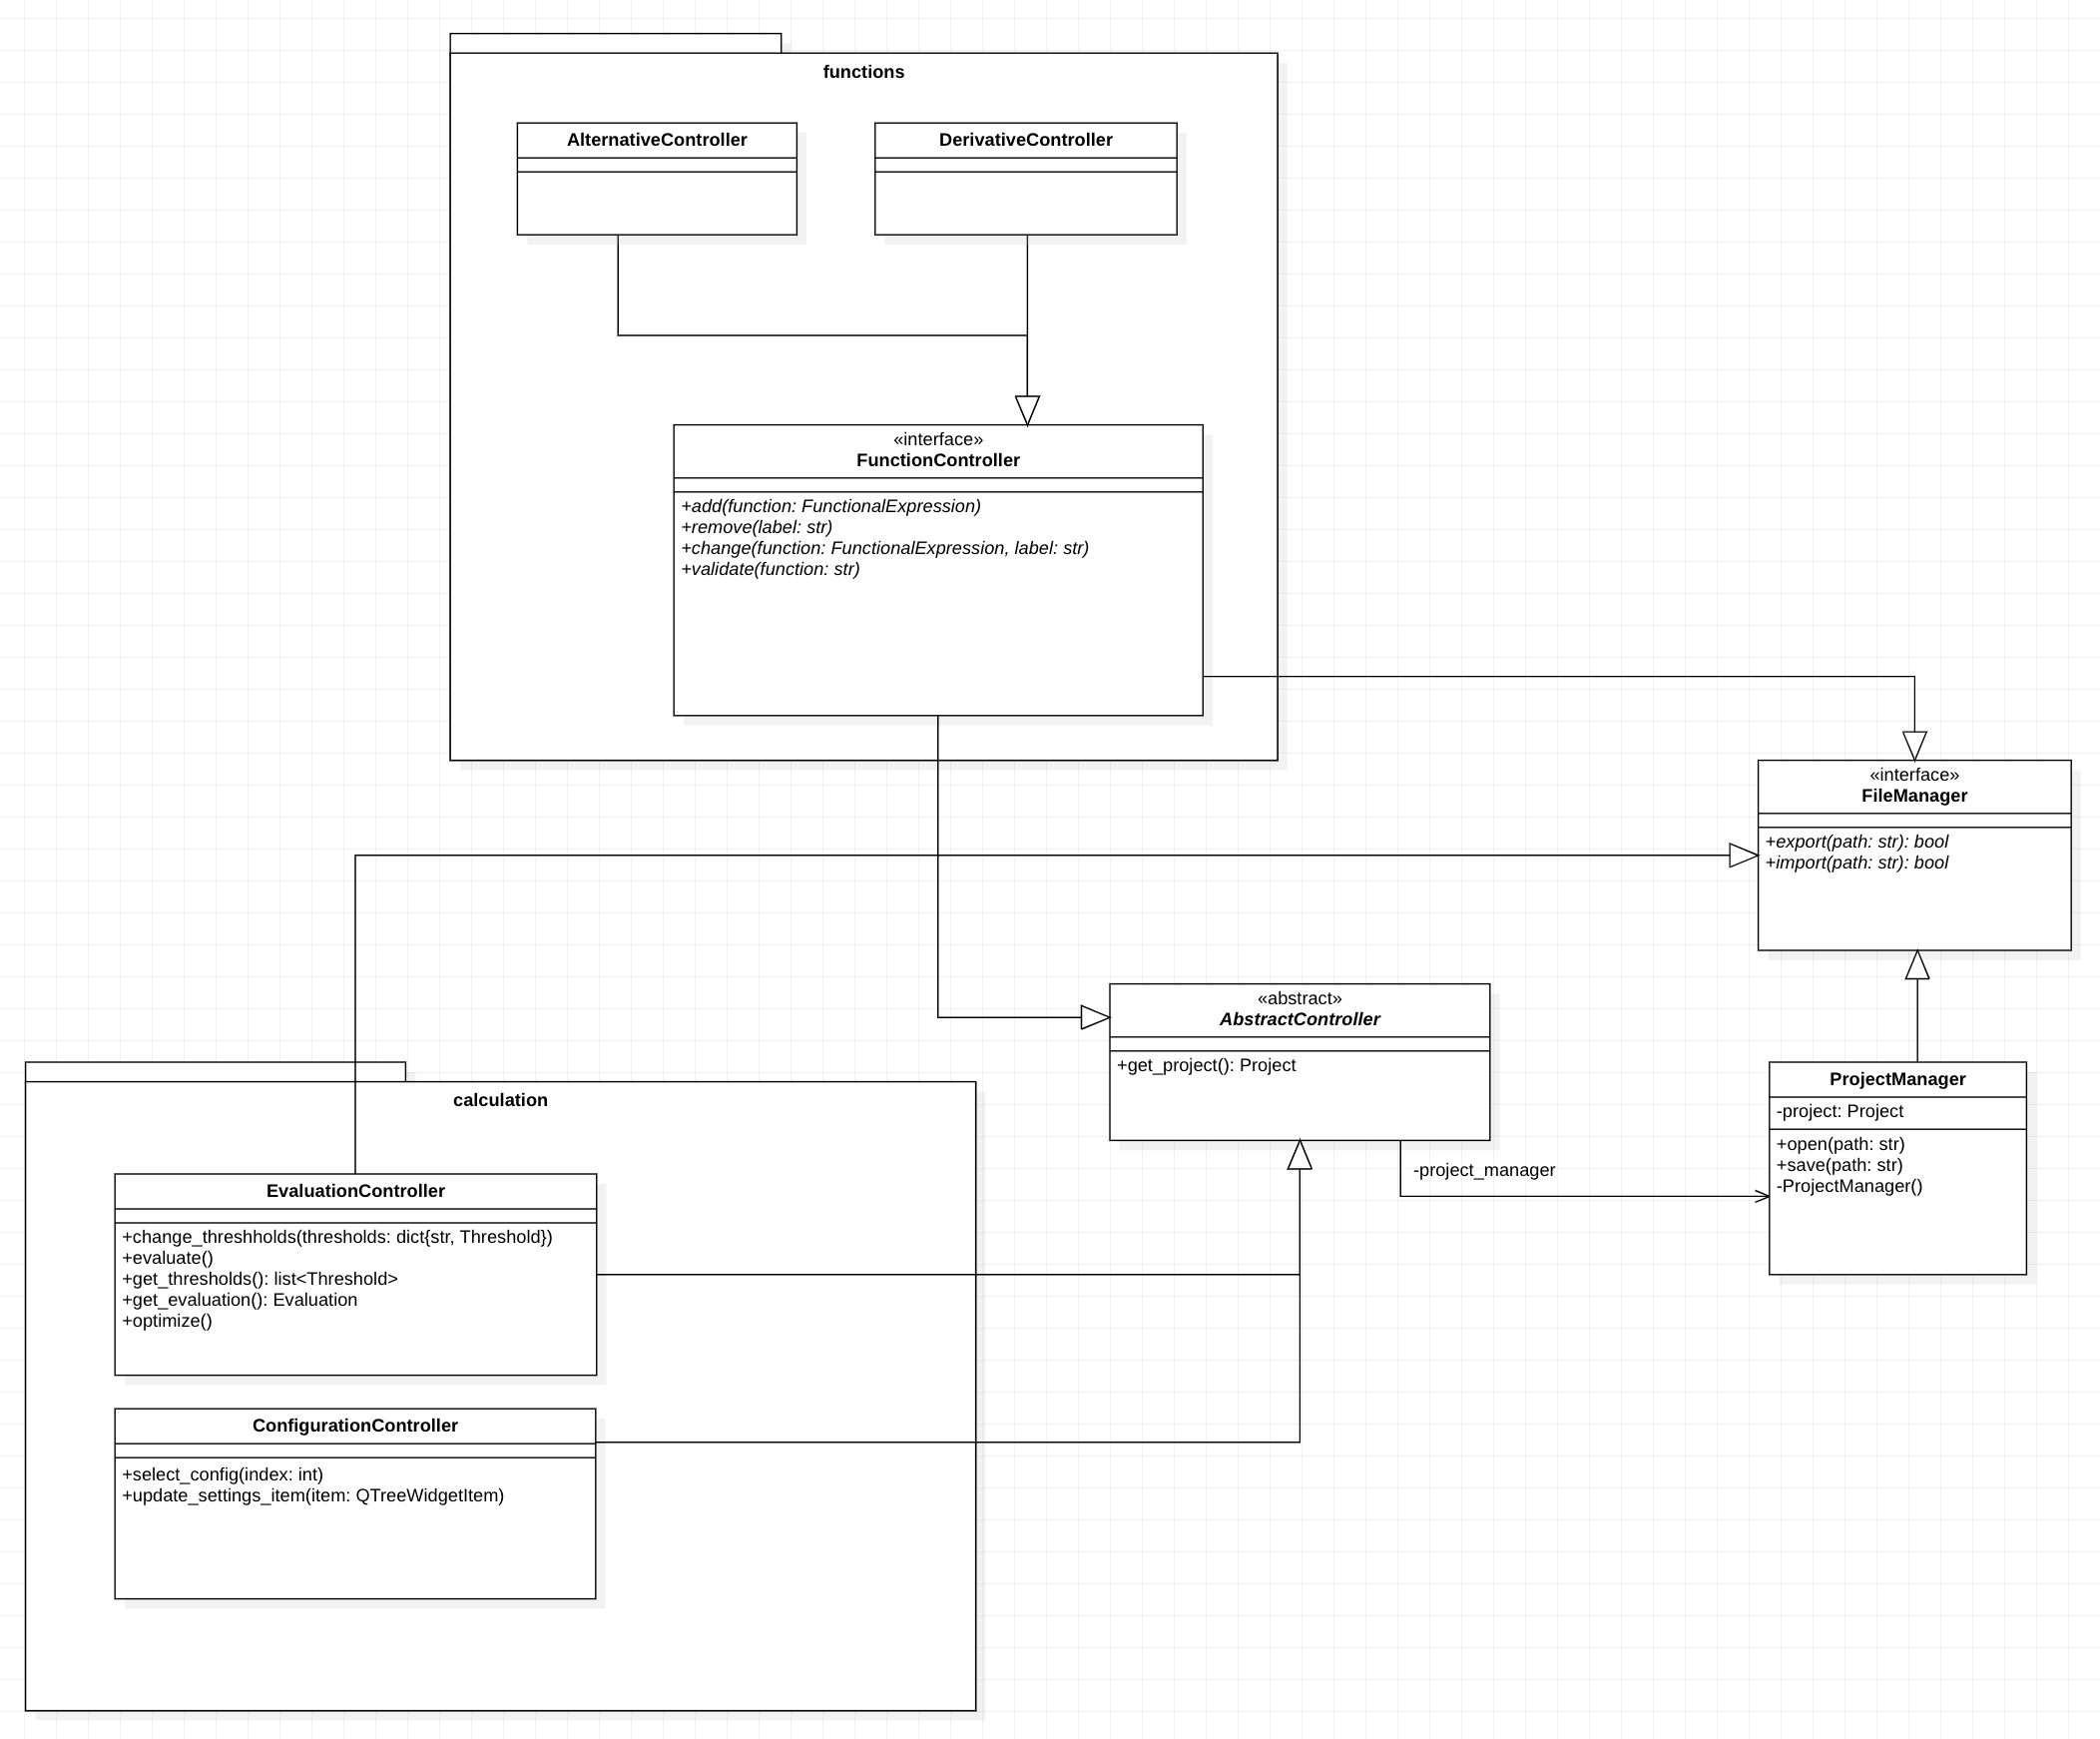
\includegraphics[width=13cm]{entwurf/Entwurf_dokument/img/Floriane/ControllerklassendiagrammTemporaer.png}
    \caption{Klassendiagramm Controller}
\end{figure}

Das Package \textit{Controller} beinhaltet sechs Klassen und zwei Interfaces, die den 'Controll'-Teil des Modells 'Model-View-Control' umsetzen.

\newpage
\textbf{\large{FileManager}}\\\\
Abbildung XY

Das Interface \textit{FileManager} dient der Interaktion mit externen Dateien. Es wird von allen Klassen im Controller implementiert.
\newline \newline
\textbf{{Methoden}}
\begin{itemize}
\item \texttt{import(path:str):bool} \newline Dient dem Import aller notwendigen Dateien und behandelt den Zugriff auf diese. Die Controller implementieren die Methode um sie für die jeweiligen Daten bzw. Funktionen zu nutzen.
\\\\
\underline{{Parameter}}

\begin{tabular}{lll}
 & \texttt{path:str} & Der Pfad zum Speicherort der zu importierenden Datei. \\
\end{tabular}

\underline{{Rückgabewert}}

\begin{tabular}{lll}
 & \texttt{bool} & Ob der Import erfolgreich war. \\
\end{tabular}


\item \texttt{export(path:str):bool} \newline Führt den Export einer Datei zu einem bestimmten Pfad aus. Diese Methode wird vom jeweiligen Controller implementiert.
\\\\
\underline{{Parameter}}

\begin{tabular}{lll}
 & \texttt{path:str} & Der Pfad zum Speicherort der zu speichernden Datei. \\
\end{tabular}

\underline{{Rückgabewert}}

\begin{tabular}{lll}
 & \texttt{bool} & Ob der Export erfolgreich war. \\
\end{tabular}
\end{itemize}

\newpage
\textbf{\large{ProjektManager}}\\\\
Abbildung XY






\section{Softwareablauf}
- sequenz und aktivitätsdiagramme
\subsection{Projektmanagement}

\begin{figure}[H]%
    \centering
    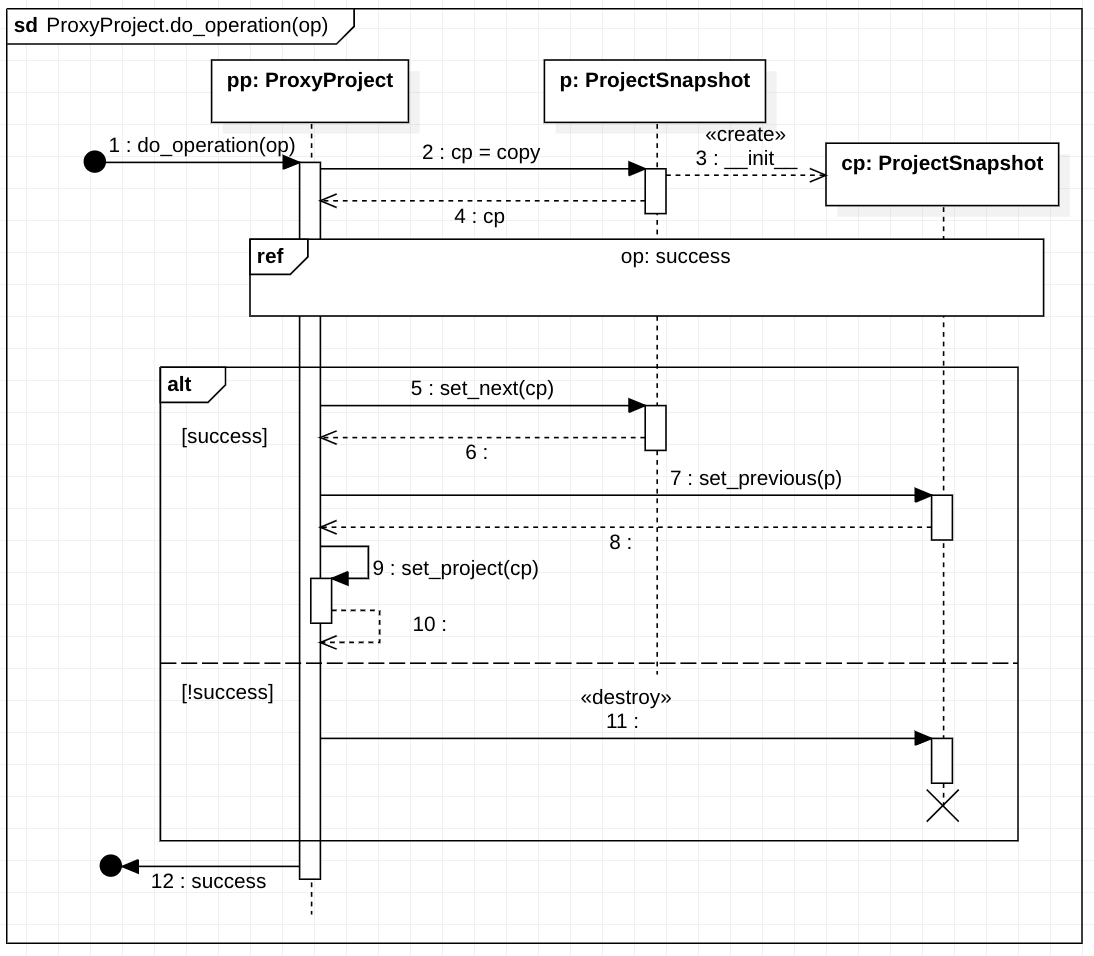
\includegraphics[width=13cm]{entwurf/Entwurf_dokument/img/Michael/sd_ProxyProject.do_operation.png}
    \caption{Sequenzdiagramm der Anwendung einer Projektoperation}
\end{figure}
TODO Beschreibung: Michael

\subsection{Attributsmanagement}
\subsection{Alternativmanagement}
\subsection{Konfiguration}
\begin{figure}[H]%
    \centering
    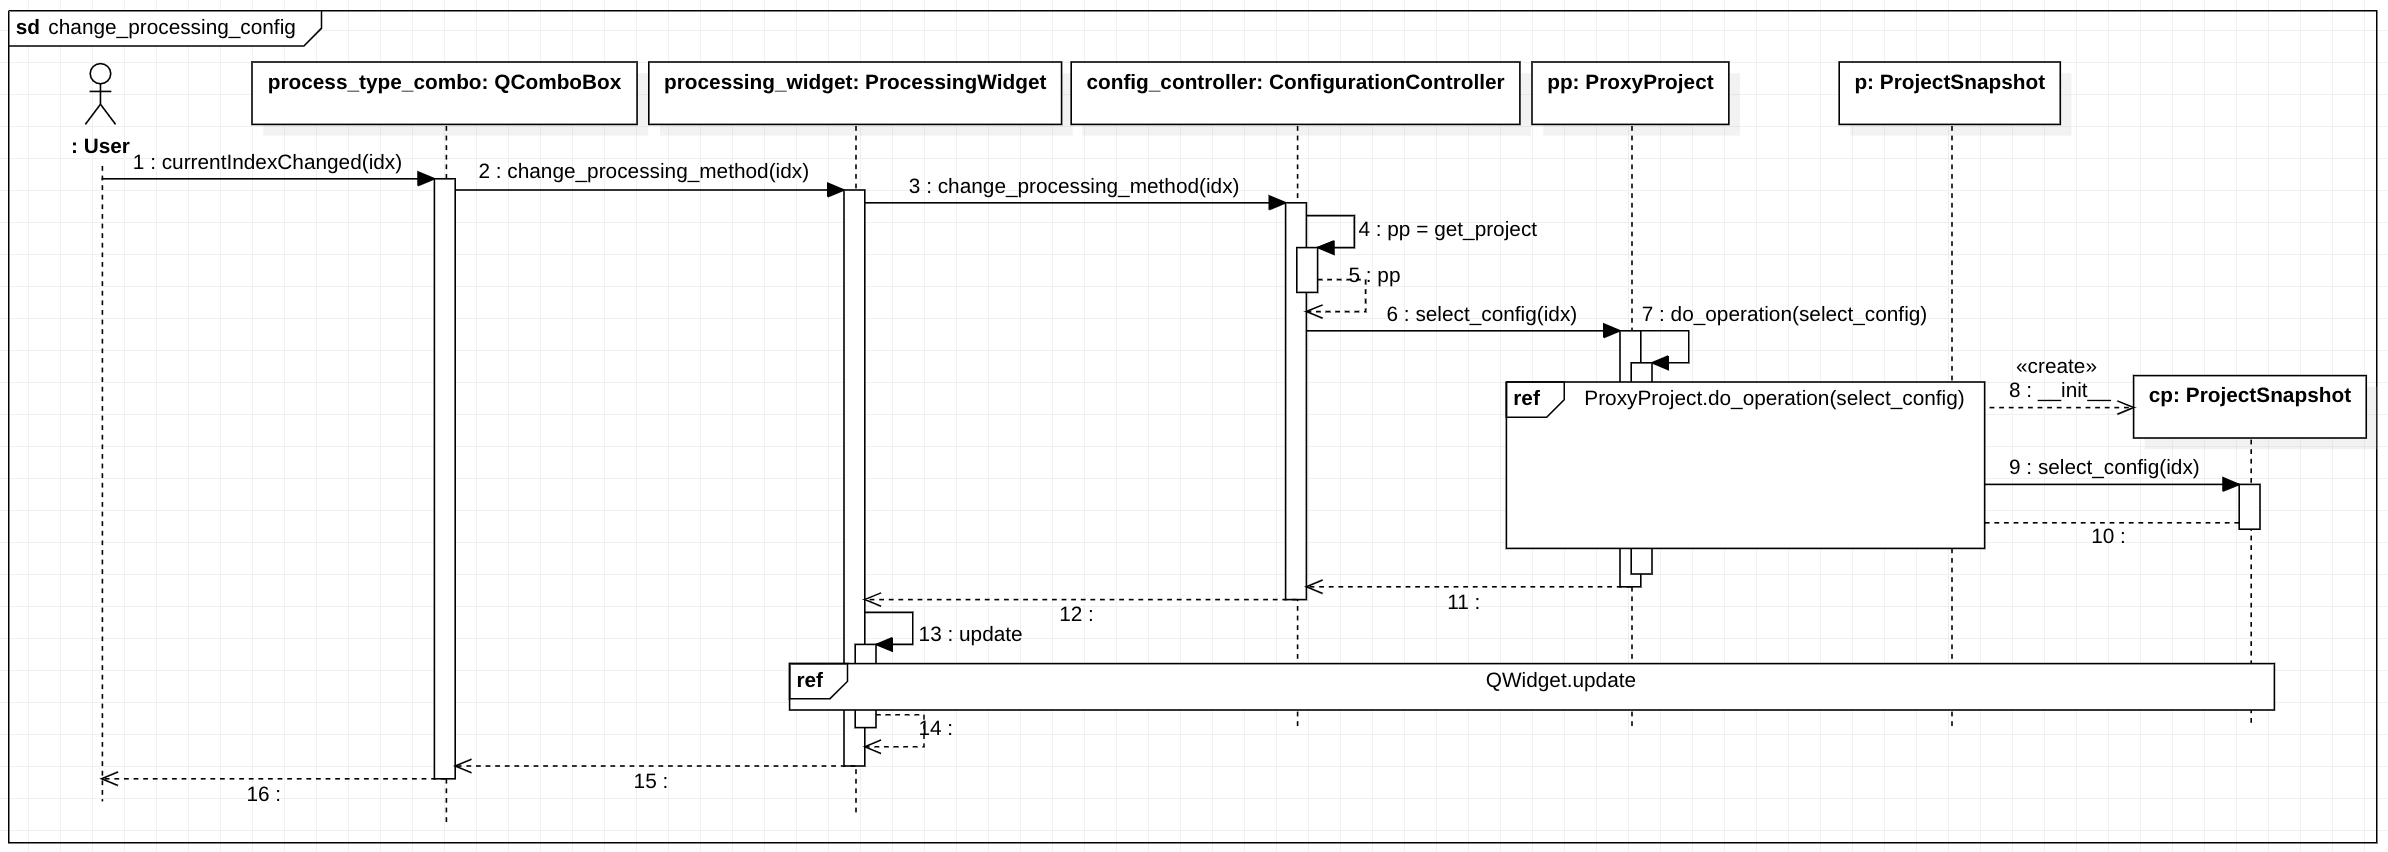
\includegraphics[width=13cm]{entwurf/Entwurf_dokument/img/Michael/sd_change_processing_config.png}
    \caption{Sequenzdiagramm der Änderung des Verarbeitungskonfigurationstyps}
\end{figure}
TODO Beschreibung: Michael

\begin{figure}[H]%
    \centering
    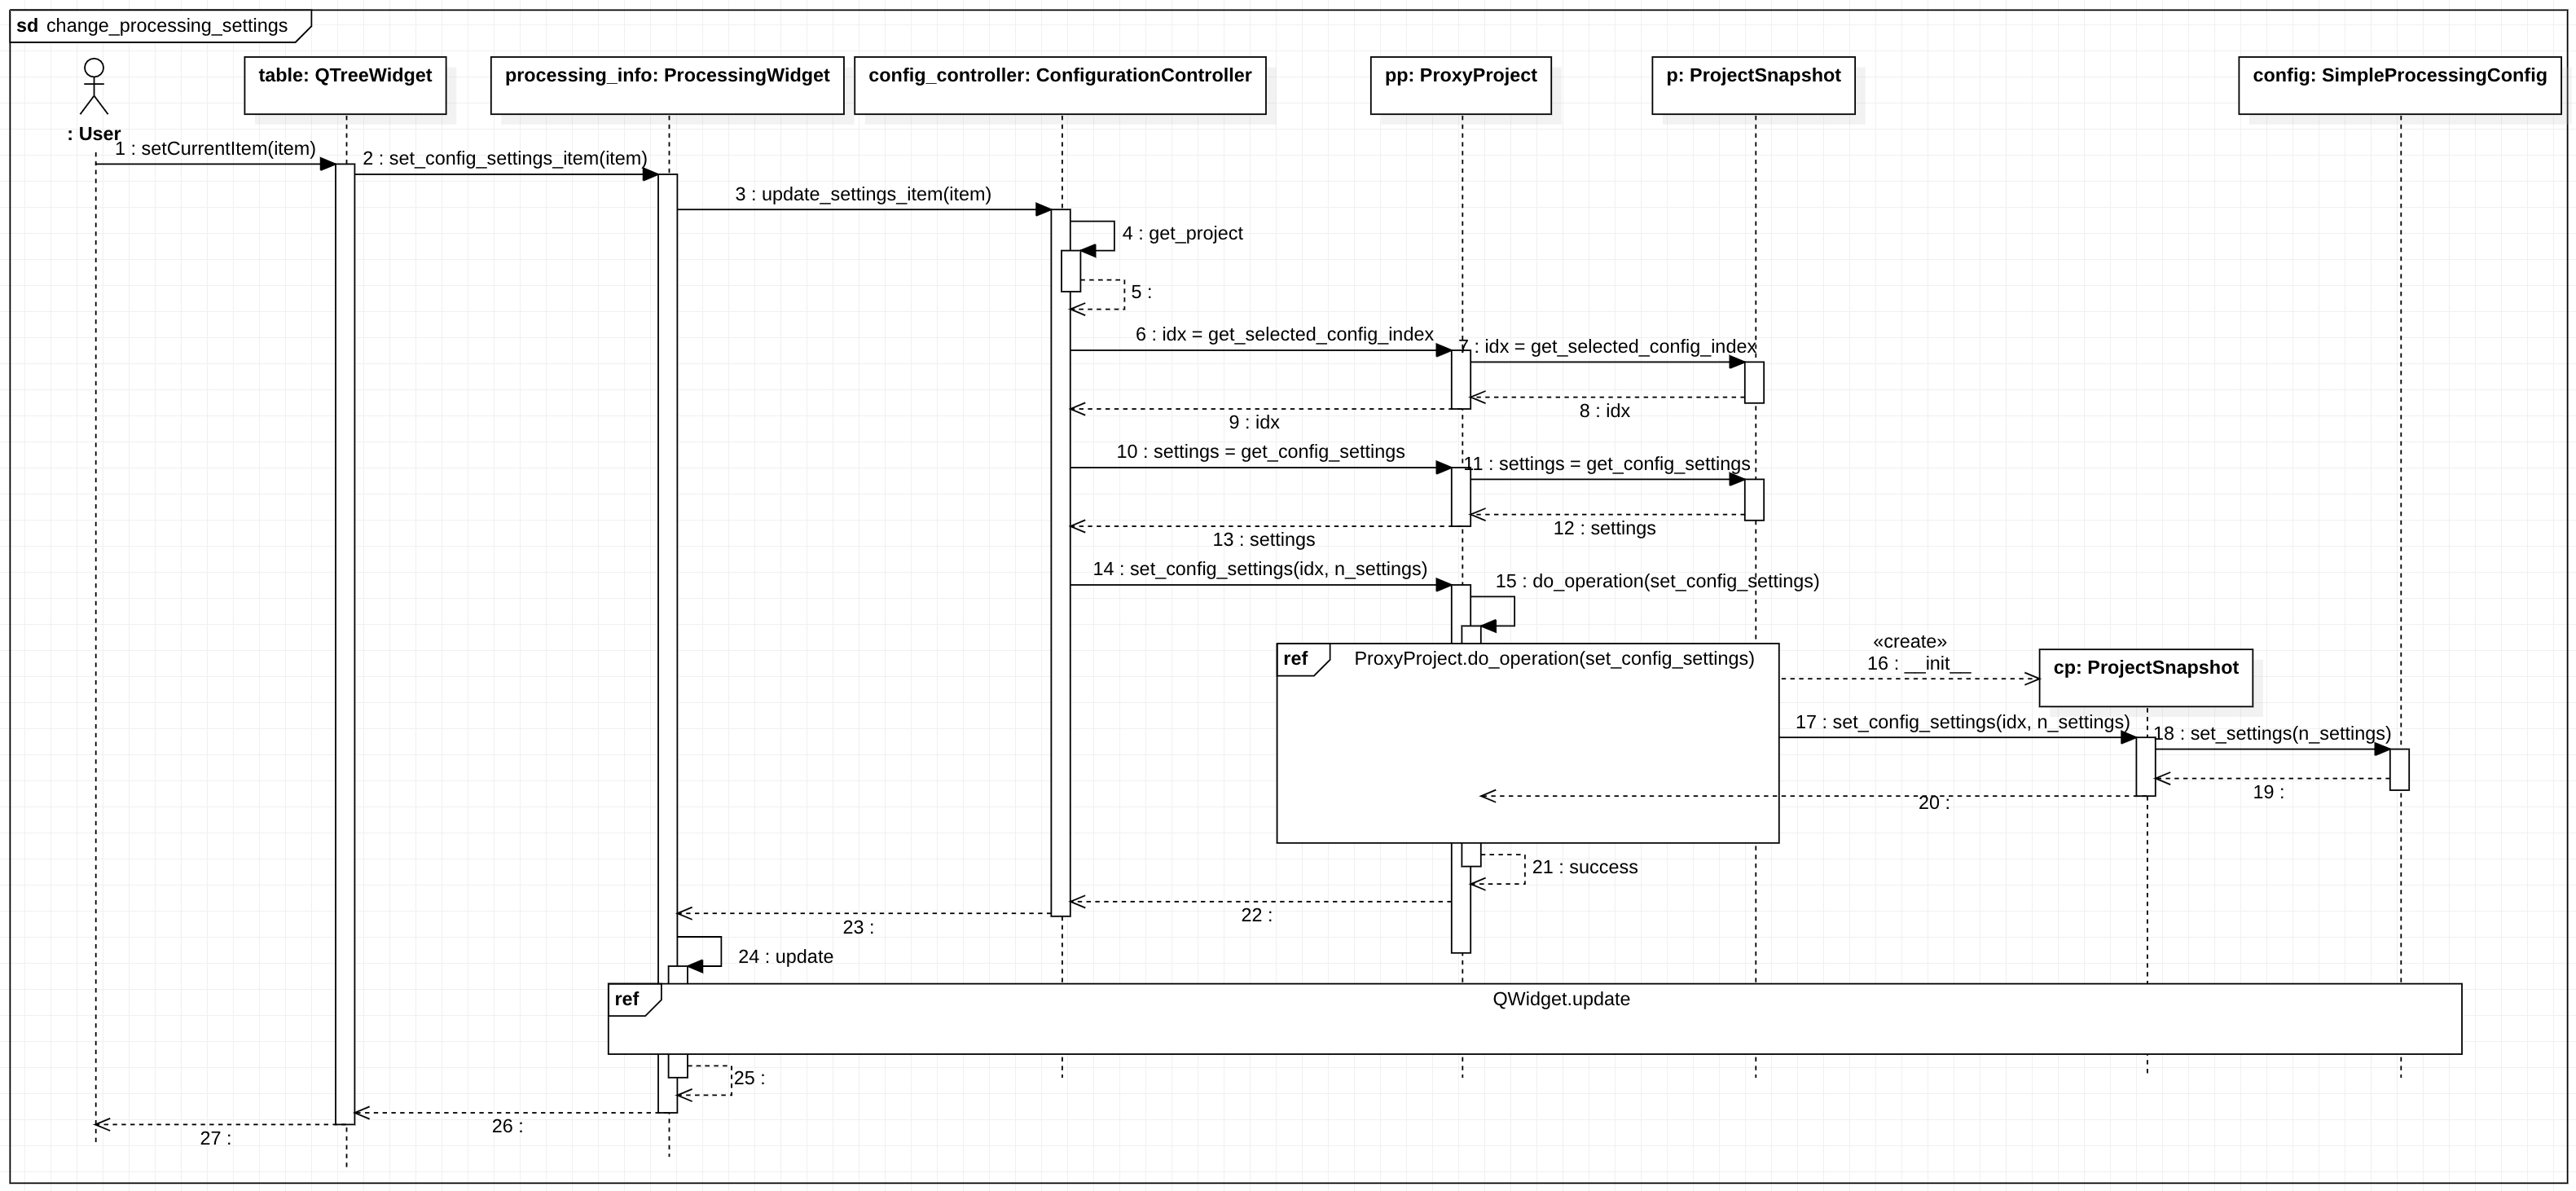
\includegraphics[width=13cm]{entwurf/Entwurf_dokument/img/Michael/sd_change_processing_settings.png}
    \caption{Sequenzdiagramm der Änderung des Einstellungen einer Verarbeitungskonfiguration}
\end{figure}
TODO Beschreibung: Michael


\subsection{Evaluation}

\begin{figure}[H]%
    \centering
    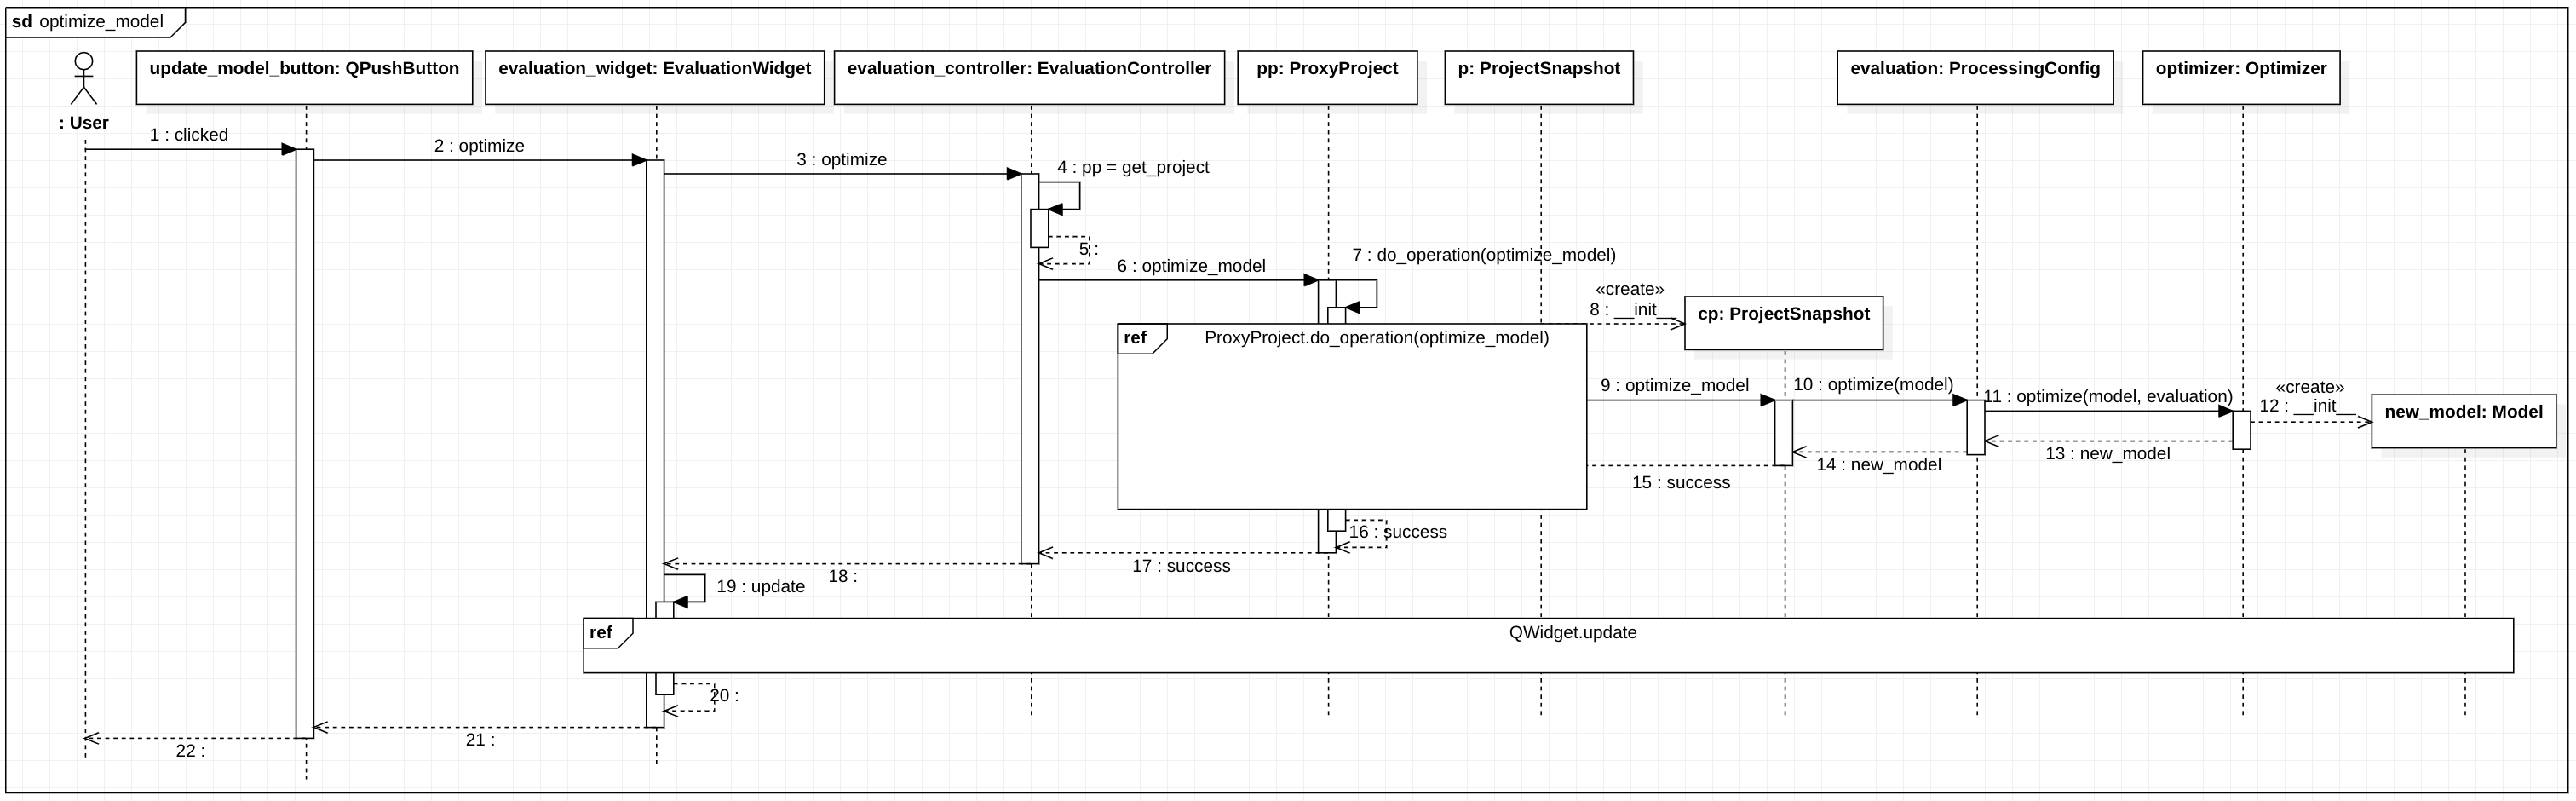
\includegraphics[width=13cm]{entwurf/Entwurf_dokument/img/Michael/sd_optimize_model.png}
    \caption{Sequenzdiagramm der Modelloptimierung}
\end{figure}
TODO Beschreibung: Michael

\section{Datenhaltung}

Der Model Builder speichert fünf verschiedene Ergebnisse: Alternativen, Attributsableitungen, Signifikanzen und Parameter, sowie die CSV-Dateien mit den zugrunde liegenden Umfragedaten und berechneten Attributen. Dabei werden Alternativen und Attributsableitungen im JSON-Format gespeichert, sodass sie in anderen Projekten widerverwertet werden können.

\subsection{Alternativen}
Die Alternativen werden als JSON-Dateien mit ihren Attributen 'label' und 'functional\_expression' gespeichert. Zusätzlich wird ebenfalls das Erstellungsdatum gespeichert.

\texttt{\begin{tabbing}
    \{\\
    \qquad"{}label": <str>,\\
    \qquad"{}functional\char`_expression": \{\\
    \qquad\qquad"{}expression": <str>\\
    \qquad\}\\
    \}
\end{tabbing}}

Das Label wird als String gespeichert und dient der Unterscheidung der einzelnen Alternativen. Das Objekt der FunctionalExpression, das im Builder verwendet wird, wird unter 'functional\_expression' als Objekt mit seinen Attributen gespeichert. In diesem befindet sich die von Python evaluierbare Funktion unter "expression", inklusive möglicher nicht-behobener Fehler.

\subsection{Attributsableitungen}
Die Attributsableitungen werden ebenfalls separat als Funktion in einer JSON-Datei gespeichert. In den Dateien befinden sich die Schlüssel 'label' und 'functional\char`_expression'. Der Schlüssel 'label' enthält den gewählten Namen der Attribtusableitung, und 'functional\_expression' enthält das Objekt aus dem Projekt im JSON-Format. Dieses enthält den Funktionasausdruck als String unter dem Schlüssel 'expression'.

\texttt{\begin{tabbing}
    \{\\
    \qquad"{}label": <str>,\\
    \qquad"{}functional\char`_expression": \{\\
    \qquad\qquad"{}expression": <str>\\
    \qquad\}\\
    \}
\end{tabbing}}
\\\\


\subsection{Umfragedaten und berechnete Attribute}
Die Umfragedaten werden auf Wunsch mit den berechneten Attributen in einer gemeinsamen CSV-Datei gespeichert. 

Dabei entsprechen die Zeilen jeweils einer berechneten Attributsableitung. Die Spaltenüberschriften entsprechen den gesetzten Namen der Attributsableitungen. 

\subsection{Parameter und Signifikanzen}
Die berechneten Parameter und Signifikanzen werden in einer CSV-Datei unter ihrem zugehörigen Variablen Namen gespeichert. Jede Zeile entspricht einer Variable aus den Nutzenfunktionen.

Die Spaltenüberschriften sind 'P' für die Spalten die Parameter enthalten und 'X' für die Spalten die die Signifikanzen enhalten. 

Die erste Spalte in der Tabelle enthält die durch die Nutzenfunktoinen festgelegten Variablennamen.


\section{Änderungen im Pflichtenheft}
- edit menu fehlt (nur undo, redo das ganze Projekt, Copy und Paste usw nur text)
- Speicherung nicht mehr zeitlich geregelt sondern schrittweise


\end{document}
